\documentclass[aps, prd, amsmath, floats, floatfix, superscriptaddress,
nofootinbib,eqsecnum]{revtex4}
\usepackage{graphicx}
\usepackage{amsmath,amssymb}
\usepackage{amsfonts}
\usepackage{xspace} % Sensible space treatment at end of simple macros
\usepackage{color}
\usepackage{dcolumn}% Align table columns on decimal point
\usepackage{bm}% bold math
\usepackage{hyperref}
\usepackage{multirow}

%\usepackage{longtable}
\special{papersize=8.5in,11in}

\def\laq{\raise 0.4ex\hbox{$<$}\kern -0.8em\lower 0.62ex\hbox{$\sim$}}
\def\gaq{\raise 0.4ex\hbox{$>$}\kern -0.7em\lower 0.62ex\hbox{$\sim$}}
\def\tablerule{\noalign {\vskip3truept\hrule\vskip3truept}}

\newcommand{\blue}{\textcolor{blue}}
\newcommand{\red}{\textcolor{red}}
\newcommand{\magenta}{\textcolor{magenta}}
\newcommand{\green}{\textcolor{green}}

\newlength{\sizeonefig}
\newlength{\sizetwofig}
\newlength{\sizeonefigb}
\newlength{\sizetwofigb}
\setlength{\sizeonefig}{0.45\textwidth}
\setlength{\sizetwofig}{0.45\textwidth}
\setlength{\sizeonefigb}{0.35\textheight}
\setlength{\sizetwofigb}{0.35\textheight}

\allowdisplaybreaks

\begin{document}

\title{A Bayesian approach to classifying authentication data}

\author{Evan Ochsner}
\email{evano@gravity.phys.uwm.edu}
\affiliation{Center for Gravitation, Cosmology and Astrophysics, University of Wisconsin-Milwaukee, Milwaukee, WI 53201, USA }

\begin{abstract}
This paper describes a code to ingest authentication log data and predict whether
each authentication attempt was a success or failure. It is based on exact enumeration over the user
and protocol information describing other ``recent'' authentication attempts.
The method worked well, correctly
predicting success or failure for $99.88\%$ of authentication attempts, including $91\%$
of the (rare) failures.
\end{abstract}

%\date{\today}

\maketitle

\section{Dataset}
\label{sec:Data}

The dataset under study is described in~\cite{akent-2015-enterprise-data,kent-2015-cyberdata1},
and can be downloaded from \url{http://csr.lanl.gov/data/cyber1/}.
We wish to classify authentication attempts and predict whether they will succeed or fail
based on the other information available. 

The data is presented as a compressed, CSV file. I split the data into files containing
one million lines each, which results in $1,051$ files (throughout, I will refer to these files as ``chunks'').
Thus, we see that the dataset contains a little over 1 billion events.
The URL above tells us the data contains events from 
$\sim 10,000$ users and $\sim 10,000$ computers.

Each line of input data consists of the following columns:
\begin{enumerate}
	\item time (an integer number of seconds)\\
	\line(1,0){50}
	\item source user@source domain
	\item destination user@destination domain
	\item source computer
	\item destination computer\\
	\line(1,0){50}
	\item authentication type
	\item logon type
	\item authentication orientation\\
	\line(1,0){50}
	\item result (Success or Fail) 
\end{enumerate}
If any of the columns are unknown for a given event, they are denoted with a question mark.
The events in the original file are ordered chronologically, and the chunks maintain this ordering.

Note that there are essentially three types of information here (in addition to the result, success or failure).
The first is the time stamp.
Next, columns 2-5 are a set I will call \emph{user} information, which describes
``who or what is involved in the attempted authentication''.
Lastly, columns 6-8 I will denote \emph{protocol} information, or ``what sort of authentication procedure is being attempted''.

To understand the data a little better, I examined the first split input file, which contains the first one million events,
or about $0.1\%$ of the full set. The data contained $993123$ successes ($99.3\%$) and $6877$ failures ($0.7\%$).
The rates of authentication events, successes and failures were rather consistent over the $\sim 3$ hour duration
of the chunk, with $\sim 100$ successful authentications and a single-digit number of failures in a typical second.
There were $82,566$ unique combinations of user and protocol information (columns 2-8). Of these, $82,310$ succeeded at least once,
$280$ failed at least once, and only $24$ had some successes and some failures within the chunk.

\begin{figure}
\label{Figure1}
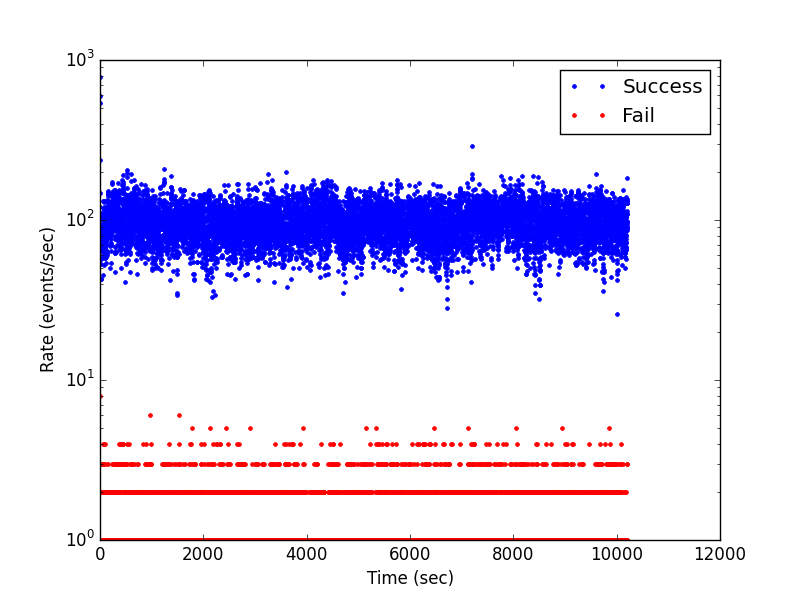
\includegraphics[width=0.75\textwidth]{rate_x00000.png}
\caption{Rate of successful and failed authentication attempts in the first data chunk.
The absolute and relative rates of success and failure remain reasonably constant over the whole chunk.}
\end{figure}

\section{Bayesian Classifier}
\label{sec:Bayes}

Bayes' theorem gives us an expression to determine the posterior probability $p(r | \vec{x} )$ of a result $r$ (success or failure),
given the other observed variables $\vec{x}$:
\begin{equation}
p(r | \vec{x}) = \frac{ p(\vec{x} | r)\ p(r) }{p(\vec{x})} \ .
\end{equation}
Here the \emph{likelihood} $p(\vec{x} | r)$ is the probability of getting the observed variables $\vec{x}$ 
if we assume the result is $r$. $p(r)$ is the prior, or our belief about the overall chances of success or failure.
The denominator $p(\vec{x})$ is the \emph{evidence},
\begin{equation}
p(\vec{x}) = \sum_r p(\vec{x} | r) \ p(r) = p(\vec{x} | S) \ p(S) + p(\vec{x} | F) \ p(F)\ .
\end{equation}
However, for our purposes, we need not worry about the evidence. We can cancel it out by working with a
\emph{Bayes factor}, in this case the relative probability of failure versus success:
\begin{equation}
B = \frac{p(F | \vec{x})}{p(S | \vec{x})} = \frac{p(\vec{x}|F) \ p(F)}{p(\vec{x} | S) \ p(S)}\ .
\end{equation}
If $B > 1$, then failure is the most likely outcome, while the opposite is true when $B < 1$ (If $B=1$,
then we consider failure and success to be equally probable). Note that this classifier does not just predict success or failure,
but quantifies the strength of that belief. Therefore, we can distinguish cases where we are confident in a result
from more marginal cases. We might flag these cases where the Bayes factor is near 1 for closer study.
We could even assign costs to each type of misclassification, and adjust the Bayes factor value
at which we change our decision. For example, if we have a very strong desire to correctly predict failures, and
do not mind a some reasonable number of false predictions of success, we could predict failure for some
Bayes factors smaller than one, say anything above 0.5 or 0.1.

Note that all of the user and protocol variables draw values from discrete, finite sets.
Therefore, at least in principle, we can consider each combination
its own unique ``user-protocol (UP) key'' and tally how many times each key has previously
succeeded or failed to estimate the probability that future attempts with that same UP key will succeed or fail.
Therefore, if $N_F(K)$ is the number of times we have seen a UP key $K$ fail, and $N_F$ is the
total number of failures observed so far, then the likelihood of failure for key $K$ is just:
\begin{equation} \label{eq:LR}
p(K|F) = N_F(K) / N_F\ .
\end{equation}
and similarly for the likelihood of success, $p(K|S)$.

Since we deal with a likelihood ratio, when $p(K|S)=0$, we are in danger of dividing by zero, and so must handle this
case specially. If $p(K|S) = p(K|F) = 0$, then we have not seen any attempts with this UP key before. The data tells
us nothing with our model of predicting based on past outcomes with the exact same parameters. 
Therefore, the data are uninformative, so we set the
likelihood ratio to 1 and our Bayes factor just becomes the prior ratio. If $p(K|S)=0$, but $p(K|F) > 0$, this means we have
seen this key fail, but have never seen it succeed. It should be clear we will predict failure in this case. The likelihood ratio
formally diverges under our model, but we can set it to some arbitrary large, finite value that will ensure we strongly predict
failure.

By inspecting the first chunk, we have reasonable guesses for the priors, $p(F)$ and $p(S)$. Additionally, we see there
are roughly $\sim 80,000$ unique UP keys. This is a manageable number to tally and track individually. Even in the worst case, where all million entries in a chunk have unique keys, this would still likely be a manageable number to tally.

It is unclear how many keys we can expect in the total set. Certainly it will grow over time and tracking all keys will become
a more expensive task by the end of the dataset, possibly so expensive as to be problematic. Therefore, it seems
sensible to track only keys from ``recent'' events and throw away information from older events. 

Even apart from 
computational issues, it may make sense to give more weight to recent events. For example, suppose one computer
intends to authenticate with another once a day. However, the connection failed when initially setup, and someone
had to debug the issue making hundreds of failed authentication attempts at the beginning. If we store all events with
equal weight, the model will predict failure until the system has worked correctly without failure for hundreds of days.
If we weighted recent events more, we might start correctly predicting success much sooner. 
One might try many time-weighting schemes and attempt to learn which fit the real-world data best.

%So, all of the work has been
%recast as finding a good model for the likelihood ratio, $p(\vec{x}|F)/p(\vec{x}|S)$. 
%Let us consider a couple special cases.

%\subsection{Naive Bayesian classification}

%If all of the variables $\vec{x}$ vary independently of one another, then the likelihood will separate into the likelihood of
%the observed value for each variable, e.g.:
%\begin{equation}
%p(\vec{x}|r) = \Pi_{i} p(x_i|r) = p(x_1|r) \times ... \times p(x_N|r)\ .
%\end{equation}
%This is a reasonable approach if we believe one or more of the variables is not correlated with the others,
%or perhaps has a rather weak correlation. Unfortunately, that is not likely to be the case for most of the variables
%in this problem. For example, presumably not all users have access to all computers, and certain computers may not support
%certain authentication actions. Therefore, there are bound to be correlations between and among the
%user and protocol variables.

%Additionally, if a computer is down for maintenance every Tuesday at Noon, that would create
%a correlation between that computer and time. However, the rates seen in Fig.~\ref{Figure1} seem consistent
%with random fluctuations about a constant average rate. In particular, there are no spikes in failures such as we might
%see if one or many computers go down for maintenance. Of course, this might appear in later chunks, but the first
%chunk suggests that at least much of the time, the chances of success or failure will not strongly correlate with time
%(i.e. remain fairly constant).

%\subsection{Classification by exact enumeration}

%Note that all of our variables come from discrete, finite sets (time is known only to within an integer and covers a finite span).
%Therefore, at least in principle, it is possible to enumerate every possible combination of variables and assign a likelihood to
%each one. In this case, that would mean every possible combination of user and protocol variables, and every possible 
%integer time in the range.

%Or, we could separate time from the other variables (since we suspect it weakly correlates to the success/fail outcome)
%and enumerate all possible combinations of user and protocol variables. We could tally up how often each combination
%succeeds or fails, and use that to compute the likelihoods for future authentication attempts with that
%combination of variables.

\section{Code Design}
\label{sec:Code}

The auth log was split into ``chunks'', separate files containing
one million lines each (chronological ordering preserved) using the {\tt split} command line tool. 

The code to process these chunks and classify each line was written by Python by defining an {\tt AuthClassifier} class.
The class reads in a chunk of the auth logs and processes each line chronologically in series.
First, the auth log line is split into three value: time $T$, a user-protocol key $K$
(columns 2-8 concatenated into a single string), and result $R$ (a string that is either $S$ or $F$).
$K$ is passed (importantly, $R$ is not passed!) to a class method to compute the likelihood ratio
in the manner described above in Eq.~\ref{eq:LR}.
This method looks up the tally for key $K$ $N_r(K)$, in dictionaries holding the counts for each key
in this and the previous chunk. Dictionary lookups are fast in Python, so this is an efficient storage scheme.
The total number of successes in this and the previous scheme are simply stored as integers. The likelihood for $R$
(either $S$ or $F$) is computed as:
\begin{equation}
p(K|R) = \frac{N_{R,curr}(K) + N_{R,prev}(K)}{N_{R,curr} + N_{R,prev}}\ ,
\end{equation}
where ``curr'' and ``prev'' denote tallies from the current and previous chunks.  
The likelihood ratio is multiplied by the prior ratio to compute the Bayes factor $B$. If $B > 1$,
it records a prediction of failure;
if $B \leq 1$, it records a prediction of success.

After the prediction is made, it then updates the tally for the total number of successes and failures in this chunk,
and updates the dictionary holding tallies of successes or failures for that key $K$ in the current chunk. 
When a chunk is completely processed, it outputs the total success/failures counts and the tally-by-key dictionaries for this
chunk into a pickle file. It also outputs a small JSON results file with the total counts and prediction results for this chunk.
It can optionally output a pickle file containing arrays of time, UP key, prediction, result, and Bayes factor for every single
event if one wishes to study a chunk in more detail.
NumPy can efficiently manipulate such arrays to transpose, count unique values, histogram, etc.

When transitioning from one chunk to another, the tally-by-key dictionaries and total counts for what was the ``current'' chunk
are moved to become the dictionaries and counts for the new ``previous'' chunk.
They can either be copied in memory (for example if running inside a loop over chunks) or loaded from the pickle file
(for example, for the first chunk in a loop). The prior ratio is estimated by reading in results files from all previous files
and dividing the total number of failures by the total number of successes. From this workflow, it should be clear that the
prior is updated only after each chunk, while the data to compute likelihood ratio is updated after every single event.

The first chunk was processed without predicting the outcome, in order to compute an initial prior ratio. All other $1,050$
chunks were processed with the results predicted as described above. The code was run on my
(quite ordinary, three-year-old) laptop and finished in roughly two hours.

\section{Results}
\label{sec:Results}

The first chunk of one million events was used as a training set to compute the prior ratio for success and failure.
The remaining one billion plus events were processed by the Bayesian classifier code and the results tallied.
The results are summarized in Table~\ref{Table1}.

%\begin{center}
%\begin{table}
%\begin{tabular}{|c|c|cc|}
%\hline
% & & \multicolumn{2}{ c |}{Prediction} \\ \hline
% & & Success & Fail \\ \hline
% \multirow{2}{*}{Result} & Success  & 98.77\% & 0.01\% \\
% & Fail  & 0.11\% & 1.11\% \\ \hline
%\end{tabular}
%\caption{Breakdown of auth events by predicted outcome and actual result.
%Note that 99.88\% of events were correctly classified.}
%\label{Table1}
%\end{table}
%\end{center}

\begin{center}
\begin{table}
\begin{tabular}{|c|c|cc|}
\hline
 & & \multicolumn{2}{ c |}{Prediction} \\ \hline
 & & Success & Fail \\ \hline
 \multirow{2}{*}{Result} & Success  & 98.75\% & 0.03\% \\
 & Fail  & 0.09\% & 1.13\% \\ \hline
\end{tabular}
\caption{Breakdown of auth events by predicted outcome and actual result.
Note that 99.88\% of events were correctly classified.}
\label{Table1}
\end{table}
\end{center}

Note that $99.88\%$ of events were correctly classified. Of the successful authentications, only about $3$ in $10,000$
was misclassified as an expected failure. Of the failed authentications, about $91\%$ were correctly predicted to be failures.
If we think of these failures as anomalies we wish to detect, then this method detected $\sim 93\%$ of the anomalies
with a false-alarm probability of $0.01\%$.


% If you have a bibliography, uncomment below and point to the .bib list of references
\bibliography{mybib}
\end{document} 

